\everymath{\displaystyle}
\documentclass{beamer}
% \documentclass[handout]{beamer}

%\usepackage[pdftex]{color,graphicx}
\usepackage{amsmath,amssymb,amsfonts}

\mode<presentation>
{
  % \usetheme{Darmstadt}
  % \usetheme[hideothersubsections]{Hannover}
  % \usetheme[hideothersubsections]{Goettingen}
  \usetheme[hideothersubsections, right]{Berkeley}

  \usecolortheme{seahorse}
  % \usecolortheme{dolphin}
  \usecolortheme{rose}
  % \usecolortheme{orchid}

  \useinnertheme[shadow]{rounded}

  \setbeamercovered{transparent}
  % or whatever (possibly just delete it)
}

\mode<handout>{
  \setbeamercolor{background canvas}{bg=black!5}
  \usepackage{pgfpages}
  \pgfpagesuselayout{4 on 1}[a4paper,border shrink=5mm, landscape]
}

\usepackage[brazilian]{babel}
% or whatever

% \usepackage[latin1]{inputenc}
\usepackage[utf8]{inputenc}
% or whatever

\usepackage{times}
%\usepackage[T1]{fontenc}
% Or whatever. Note that the encoding and the font should match. If T1
% does not look nice, try deleting the line with the fontenc.


\title%[] % (optional, use only with long paper titles)
{Etapas da Pesquisa}

\subtitle
{Planejamento, Buscas e Perdas} % (optional)

\author%[] % (optional, use only with lots of authors)
{Felipe Figueiredo}% \and S.~Another\inst{2}}
% - Use the \inst{?} command only if the authors have different
%   affiliation.

\institute[] % (optional, but mostly needed)
{
}
  % \inst{1}%
  % Department of Computer Science\\
  % University of Somewhere
  % \and
  % \inst{2}%
  % Department of Theoretical Philosophy\\
  % University of Elsewhere}
% - Use the \inst command only if there are several affiliations.
% - Keep it simple, no one is interested in your street address.

\date%[] % (optional)
{}

% \subject{Talks}
% This is only inserted into the PDF information catalog. Can be left
% out. 



% If you have a file called "university-logo-filename.xxx", where xxx
% is a graphic format that can be processed by latex or pdflatex,
% resp., then you can add a logo as follows:

\pgfdeclareimage[height=1.6cm]{university-logo}{../logo}
\logo{\pgfuseimage{university-logo}}



% Delete this, if you do not want the table of contents to pop up at
% the beginning of each subsection:
\AtBeginSubsection[]
%\AtBeginSection[]
{
  \begin{frame}<beamer>{Sumário}
    \tableofcontents[currentsection,currentsubsection]
  \end{frame}
}


% If you wish to uncover everything in a step-wise fashion, uncomment
% the following command: 

\beamerdefaultoverlayspecification{<+->}


\begin{document}

\begin{frame}
  \titlepage
\end{frame}

\begin{frame}{Sumário}
  \tableofcontents
  % You might wish to add the option [pausesections]
\end{frame}


%% Template
% \section{}

% \subsection{}

% \begin{frame}{}
%   \begin{itemize}
%   \item 
%   \end{itemize}
% \end{frame}

% \begin{frame}
%   \begin{columns}
%     \begin{column}{5cm}
%     \end{column}
%     \begin{column}{5cm}
%     \end{column}
%   \end{columns}
% \end{frame}

% \begin{frame}{}
%   \includegraphics[height=0.4\textheight]{file1}
%   \includegraphics[height=0.4\textheight]{file2}
%   \includegraphics[height=0.4\textheight]{file3}
%   \begin{figure}
%     \caption{}
%   \end{figure}
% \end{frame}

% \begin{frame}{}
%   \begin{definition}
%   \end{definition}
%   \begin{example}
%   \end{example}
%   \begin{block}{Exercício}
%   \end{block}
% \end{frame}

\section{Planejamento}

\subsection{Preparação da Pesquisa}

\subsection{Fases da Pesquisa}

\subsection{Execução da Pesquisa}

\subsection{Relatório da Pesquisa}



\section{Buscas}

\subsection{Google Scholar}


\section{Fracassos}

\subsection{Fracassos?}

\begin{frame}{Rejeição}
  \begin{itemize}
  \item Diversos motivos podem levar à rejeição do texto
  \item Revisão por pares = escrutínio de todos os detalhes
  \item Análise da metodologia e argumentação
  \item Detecção de possíveis fraudes
  \end{itemize}
\end{frame}

\begin{frame}{O {\em peer review} não é perfeito}
  \begin{itemize}
  \item Somos todos humanos:
    \begin{itemize}
    \item rejeição por motivos pessoais
    \item ideologia
    \end{itemize}
  \item Falha na revisão
  \item Aceitação de estudos {\em fake}
  \item Rejeição de estudos {\em válidos}
  \end{itemize}
\end{frame}

\begin{frame}{Preconceito}
  Artigo rejeitado pois as autoras eram mulheres, não havia nenhum
  homem no grupo
    \begin{block}{O revisor}
      \ldots find one or two male biologists to work with (or at least
      obtain internal peer review from, but better yet as active
      co-authors), in order to serve as a possible check against
      interpretations that may sometimes be drifting too far away from
      empirical evidence into ideologically based assumptions.
    \end{block}

\url{http://retractionwatch.com/2015/04/29/its-a-mans-world-for-one-peer-reviewer-at-least/}
\end{frame}

\begin{frame}{Preconceito}
  Artigo rejeitado pois as autoras eram mulheres, não havia nenhum
  homem no grupo
    \begin{block}{A revista}
      PLOS regrets the tone, spirit and content of this particular
      review. We take peer review seriously and are diligently and
      expeditiously looking into this matter. The appeal is in
      process. PLOS allows Academic Editors autonomy in how they
      handle manuscripts, but we always follow up if concerns are
      raised at any stage of the process. Our appeals policy also
      means that any complaints of the review process can be fully
      addressed and the author given opportunity to have their paper
      re-reviewed.
    \end{block}

\url{http://retractionwatch.com/2015/04/29/its-a-mans-world-for-one-peer-reviewer-at-least/}
\end{frame}

\begin{frame}{Ou seja...}
  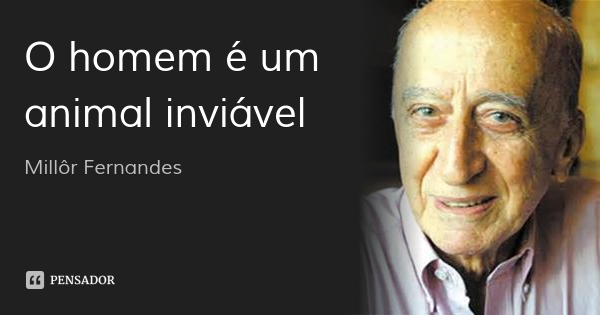
\includegraphics[width=\textwidth]{millor}
\end{frame}

\begin{frame}{Aceitação de estudos {\em fake}}
  \begin{itemize}
  \item Caso Sokal
  \item Caso Bohannon
  \end{itemize}
\end{frame}

\begin{frame}{O caso Sokal}
  \begin{itemize}
  \item Alan Sokal (físico) publicou em 1996 um estudo na {\em Social
      Text}
  \item Criticava a qualidade dos artigos nas áreas sociais, que
    usavam indevidamente argumentos matemáticos ou físicos
  \item Submeteu um artigo que argumentava que a {\em gravidade
      quântica} tinha implicações políticas profundas
  \item Citou muitos autores reconhecidos da área, e que publicavam na
    revista
  \item Aceito para uma edição especial
  \end{itemize}
\end{frame}

\begin{frame}{O caso Sokal}
  \begin{itemize}
  \item O estudo era {\em fictício}!
  \item A argumentação era incoerente
  \item as analogias eram inválidas
  \item as citações e referências estavam fora de contexto
  \item O texto foi escrito como um {\bf trote}!
  \item Posteriormente, Sokal e Jean Bricmont publicaram um livro
    ({\em Impostures Intellectuelles}) expandindo esse tipo de crítica
    ao abuso de idéias científicas
  \end{itemize}
\end{frame}

\begin{frame}{John Bohannon}
  \begin{itemize}
  \item Em 2013 John Bohannon escreveu um artigo com sérias falhas
    metodológicas
  \item Objetivo: testar o controle de qualidade em diversas revistas
    online
  \item Resultado: 304 submissões, 157 aceites, 98 rejeitas
  \end{itemize}
  \begin{block}{}
    Any reviewer with more than a high-school knowledge of chemistry
    and the ability to understand a basic data plot should have
    spotted the paper's short-comings immediately. Its experiments are
    so hopelessly flawed that the results are meaningless.
  \end{block}
  \url{http://www.sciencemag.org/content/342/6154/60.full}
\end{frame}

\begin{frame}{Esses casos são exceção!}
  \begin{itemize}
  \item Problemas existem em qualquer aspecto da humanidade
  \item Esses casos emblemáticos são notícia (leia: raros!)
  \item O processo de {\em peer review} tradicional, embora não seja
    perfeito, é responsável pelo avanço do conhecimento nas mais
    diversas áreas do conhecimento
  \item Esse processo rejeita mais trabalhos do que aceita
  \item Como lidar com a rejeição?
  \end{itemize}
\end{frame}

\begin{frame}{8 motivos comuns para rejeição}
  \url{http://www.elsevier.com/connect/8-reasons-i-rejected-your-article}
  \begin{enumerate}
  \item Não passa pelo crivo técnico
  \item Fora do escopo
  \item Incompleto
  \item Problemas metodológicos ou de análise
  \item Conclusão não segue dos resultados
  \item Pequena extensão de artigo prévio
  \item Texto incompreensível
  \item {\em Boring}
  \end{enumerate}
\end{frame}


\begin{frame}{Crivo técnico}
  \begin{itemize}
  \item Suspeita de plágio, ou está sendo analisado por outra revista
  \item Rascunho pode faltar elementos como título, autores,
    afiliações, etc
  \item Figuras ilegíveis ou incompletas
  \item Referências podem estar incompletas, ou muito antigas
  \end{itemize}
\end{frame}

\begin{frame}{Escopo}
  \begin{itemize}
  \item Estudo pode não estar dentro do escopo ou objetivos da revista
  \item Exemplo: Para a revista {\em Carbon} o material utilizado pode
    conter carbono, mas não é carbono
  \item O estudo usa carbono, mas o foco é em algo diferente
  \item Não há inovação para a área do Carbono
  \end{itemize}
\end{frame}

\begin{frame}{Incompleto}
  \begin{itemize}
  \item O estudo contém observações, mas não é um estudo completo
  \item Discussão relaciona com descobertas de outras áreas, mas não
    todas as áreas relevantes
  \end{itemize}
\end{frame}

\begin{frame}{Metodologia ou Análise de dados}
  \begin{itemize}
  \item O procedimento não inclui um grupo controle rigorosamente
    monitorado
  \item A metodologia não é reprodutível
  \item A análise não é estatísticamente válida, ou não está de acordo
    com os padrões estabelecidos na área
  \end{itemize}
\end{frame}

\begin{frame}{{\em non sequitur}}
  As conclusões não podem ser justificadas a partir dos resultados
  \begin{itemize}
  \item Argumentos ilógicos, mal estruturados ou inválidos
  \item Os dados (evidências) não suportam as conclusões
  \item As conclusões ignoram outros resultados da literatura
  \end{itemize}
\end{frame}

\begin{frame}{Pequeno incremento}
  É apenas uma {\bf pequena} extensão de um artigo anterior,
  possivelmente pelos próprios autores
  \begin{itemize}
  \item Descobertas são um pequeno incremento, e não acrescentam ao
    conhecimento da área
  \item O artigo é visivelmente parte de um estudo maior, {\em
      picotado} na maior quantidade de artigos possível
  \end{itemize}
\end{frame}

\begin{frame}{Texto incompreensível}
  \begin{itemize}
  \item Linguagem, estrutura do texto ou figuras são problemáticas
  \item Deve-se sempre mostrar o rascunho a alguém que seja fluente ou
    nativo em Inglês.
  \end{itemize}
\end{frame}

\begin{frame}{Desinteressante}
  \begin{itemize}
  \item Apenas mostra novos dados, é incremental ou de interesse
    marginal na área
  \item A pergunta do trabalho não é do interesse da área
  \item O texto não desperta interesse do público alvo da área
  \end{itemize}
\end{frame}

% \begin{frame}{10 regras simples para publicar}
%   \begin{itemize}
%   \item 
%   \end{itemize}
%   \url{http://journals.plos.org/ploscollections/article?id=10.1371/journal.pcbi.0010057}
% \end{frame}

\end{document}
